\documentclass[12pt, letterpaper]{article}
\usepackage[utf8]{inputenc}
\usepackage{pgfplots}

\title{Image Classification}
\author{
  Vasishta Kalinadhabhotla, Jing Yang, and Parth Mehrotra
}

\begin{document}
\maketitle
\section{Introduction}
  The intention of this project was to compare and contrast two classification algorithms: the Naive Bayes classifier, and the Perceptron classifier. Both algorithms were implemented primarily in Python using only standard libraries included with Python. The experiments were conducted for two different image data sets: digits and faces. Each experiment using the classifiers was tested by training 10\%, 20\%, 30\%, 40\%, 50\%, 60\%, 70\%, 80\%, 90\%, and 100\% of the training data incrementally with a sample size of 5. The results were then averaged, and the standard deviation of the results were calculated. \\ 
\section{Naive Bayes Classifier}
  Naive bayes classifier is based on the Bayes theorem. It works by calculating the probability for each possible label using conditional probability of all features for certain label. In the training process, we count the number of occurrences of each value, and divide it by the total number of all values. This will be used as conditional probability for this value for the feature (in this assignment a feature is a pixel). In classifying phase, we calculate the joint distribution of each label value. The label with highest probability with given features is the predicted value. \\ 
    When we measure the performance of the classifier against the digits dataset, we immediately began to see a very high degree of accuracy with only 20\% of the training data (figure 4.1.1). For a more complex dataset like the faces dataset we require at least 40\% of the training data to start performing at acceptable levels (figure 4.2.1). This might be due to the nature of how complex the faces data set is in comparison to the digits one. \\

\section{Perceptron Classifier}
The perceptron classifier was designed as essentially a fully connected neural network with an input layer and an output layer. Each pixel signified an input where \# and + characters were quantified with a value of 1.0, and whitespace characters were quantified with a value of 0.0. Every one of these inputs were connected to each perceptron, and there was one perceptron for each potential output of the classifier ([0, 1, 2, 3, 4, 5, 6, 7, 8, 9] for digit images, and [0, 1] for face images). During the training phase, when the classifier loaded an image, it quantified the pixels and fed them to the input layer. The inputs were then multiplied by the weights associated with the connections between an input node, and an output node. These values were then totaled at the output layer, and the final output of the classifier was decided to be the output node with the greatest total sum. If this output agreed with the associated label, then the classifier simply went onto the next image. If there was a discrepancy, the weights connecting all inputs to the output associated with the correct answer was updated according to the values given as input. \\
This design allows for the classifier to increase the weights corresponding to the inputs that coerce a correct output proportional to the value of the input. On the other hand, it also negatively impacts the connections between inputs that correspond to the incorrect output during training. One thing we have noticed is that since the final output depends on the relationship between outputs, the values that are given to the input themselves do not matter, rather it is the relationship between them that matters. Therefore it can be said that increasing training data of the same type does not benefit this classifier after a certain point, but the detail contained within the data would provide a greater benefit. Greater detail means that the relationship between the values in the pixels varies more greatly than the provided data set that only varies between 3 characters, which only translate (in this model) to two values (1.0 for \# or +, and 0.0 for whitespace). This accounts for the plateau that occurs and can be seen in Figure x below. \\

\section{Plots}
\subsection{Digit Plots}
\subsubsection{Digit Mean Accuracy}
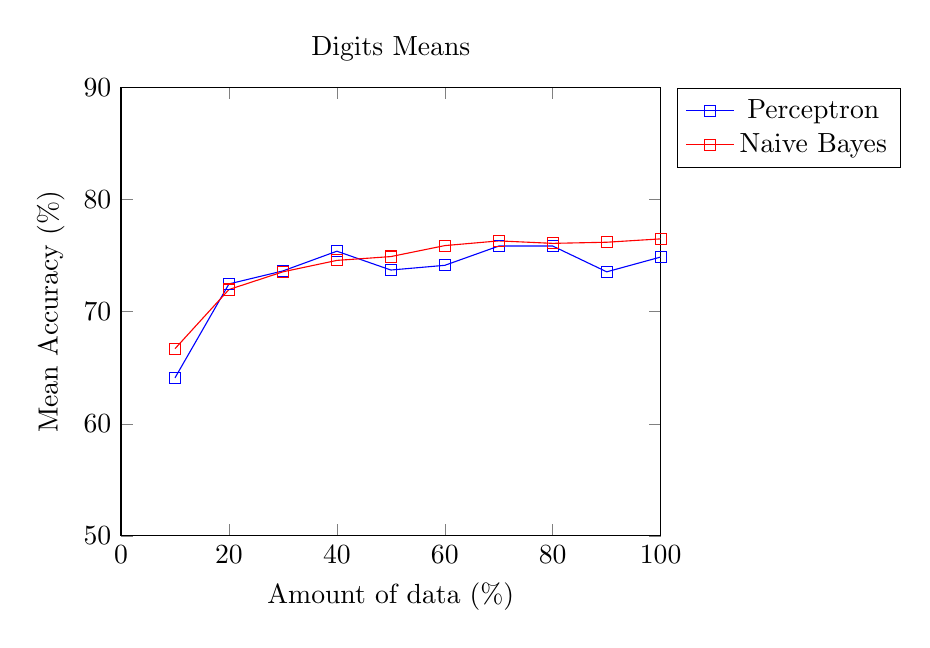
\begin{tikzpicture}
\begin{axis}[
  title={Digits Means}, 
  xlabel={Amount of data (\%)},
  ylabel={Mean Accuracy (\%)},
  xmin=0, xmax=100,
  ymin=50, ymax=90,
  legend pos=outer north east
  ]

  \addplot[
    color=blue,
    mark=square
  ]
  coordinates {
    (10, 64.1) (20, 72.47999999999999) (30, 73.64000000000001) (40, 75.39999999999999) (50, 73.72) (60, 74.14000000000001) (70, 75.86) (80, 75.86) (90, 73.55999999999999) (100, 74.88)
  };
  \addplot[
    color=red,
    mark=square
  ]
  coordinates {
    (10, 66.70000000000002) (20, 71.97999999999999) (30, 73.55999999999999) (40, 74.58) (50, 74.92) (60, 75.9) (70, 76.32000000000001) (80, 76.1) (90, 76.2) (100, 76.5)
  };
  \legend{Perceptron, Naive Bayes}

\end{axis}
\end{tikzpicture}

\subsubsection{Digit Times}
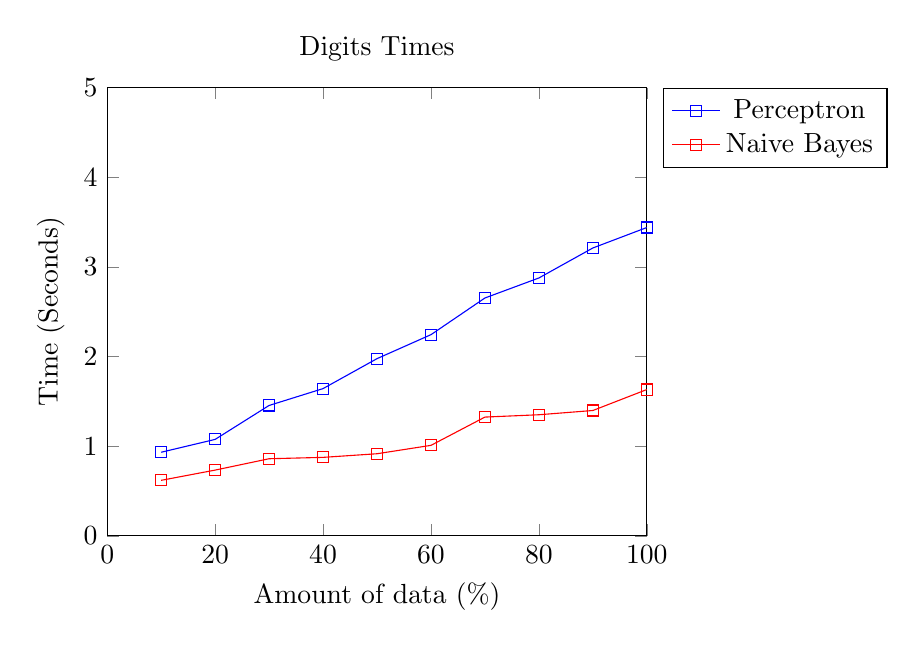
\begin{tikzpicture}
\begin{axis}[
  title={Digits Times}, 
  legend pos=outer north east,
  xlabel={Amount of data (\%)},
  ylabel={Time (Seconds)},
  xmin=0, xmax=100,
  ymin=0, ymax=5
  ]

  \addplot[
    color=blue,
    mark=square
  ]
  coordinates {
  (10,0.932571411133) (20,1.07591972351) (30,1.45445799828) (40,1.6424642086) (50,1.97654452324) (60,2.24406299591) (70,2.65311741829) (80,2.8764354229) (90,3.21098661423) (100,3.43924260139) 
  };
  \addplot[
    color=red,
    mark=square
  ]
  coordinates {
  (10,0.619478559494) (20,0.733560180664) (30,0.860241985321) (40,0.875538825989) (50,0.916040468216) (60,1.00955305099) (70,1.32490859032) (80,1.35088400841) (90,1.3982530117) (100,1.63210082054) 
  };
  \legend{Perceptron, Naive Bayes}

\end{axis}
\end{tikzpicture}

\subsubsection{Digit Std Dev}
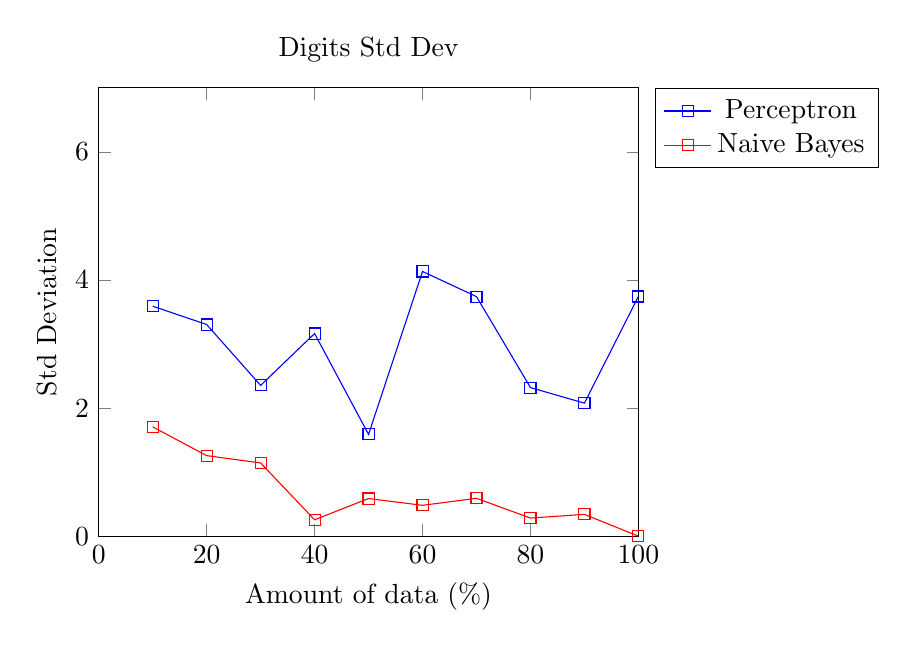
\begin{tikzpicture}
\begin{axis}[
  legend pos=outer north east,
  title={Digits Std Dev}, 
  xlabel={Amount of data (\%)},
  ylabel={Std Deviation},
  xmin=0, xmax=100,
  ymin=0, ymax=7
  ]

  \addplot[
    color=blue,
    mark=square
  ]
  coordinates {
  (10,3.59165699921) (20,3.30478441052) (30,2.35423023513) (40,3.1641744579) (50,1.58921364203) (60,4.13308601411) (70,3.74090898045) (80,2.32) (90,2.07711338159) (100,3.74240564343) 
  };
  \addplot[
    color=red,
    mark=square
  ]
  coordinates {
  (10,1.70645832062) (20,1.25761679378) (30,1.14297856498) (40,0.256124969497) (50,0.587877538268) (60,0.481663783152) (70,0.591269819964) (80,0.282842712475) (90,0.340587727319) (100,0.0) 
  };
  \legend{Perceptron, Naive Bayes}

\end{axis}
\end{tikzpicture}

\subsection{Faces}
\subsubsection{Faces Mean Accuracy}
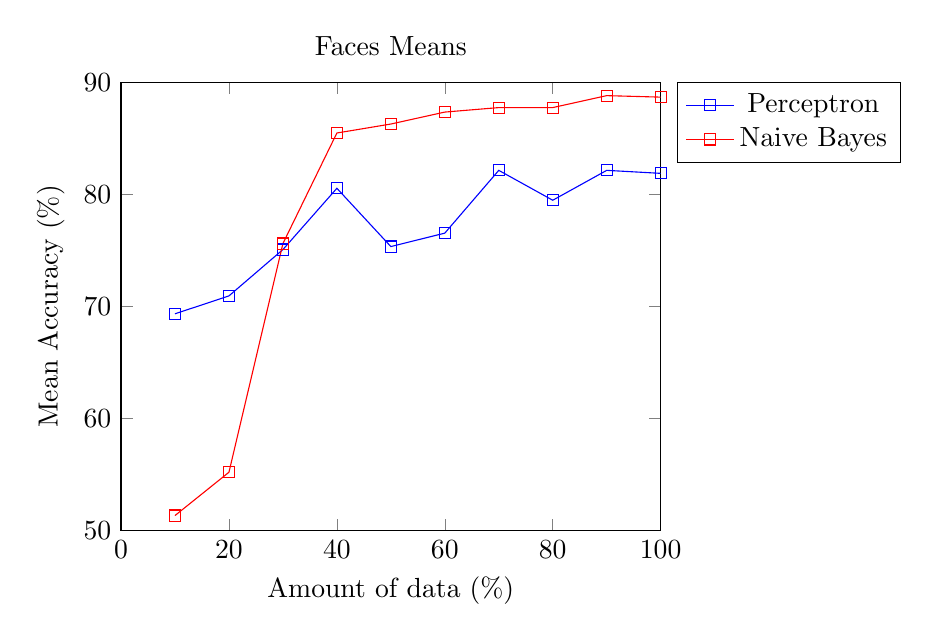
\begin{tikzpicture}
\begin{axis}[
  legend pos=outer north east,
  title={Faces Means}, 
  xlabel={Amount of data (\%)},
  ylabel={Mean Accuracy (\%)},
  xmin=0, xmax=100,
  ymin=50, ymax=90
  ]

  \addplot[
    color=blue,
    mark=square
  ]
  coordinates {
  (10,69.3333333333) (20,70.9333333333) (30,75.0666666667) (40,80.5333333333) (50,75.3333333333) (60,76.5333333333) (70,82.1333333333) (80,79.4666666667) (90,82.1333333333) (100,81.8666666667) 
  };
  \addplot[
    color=red,
    mark=square
  ]
  coordinates {
  (10,51.3333333333) (20,55.2) (30,75.6) (40,85.4666666667) (50,86.2666666667) (60,87.3333333333) (70,87.7333333333) (80,87.7333333333) (90,88.8) (100,88.6666666667) 
  };
  \legend{Perceptron, Naive Bayes}

\end{axis}
\end{tikzpicture}

\subsubsection{Faces Times}
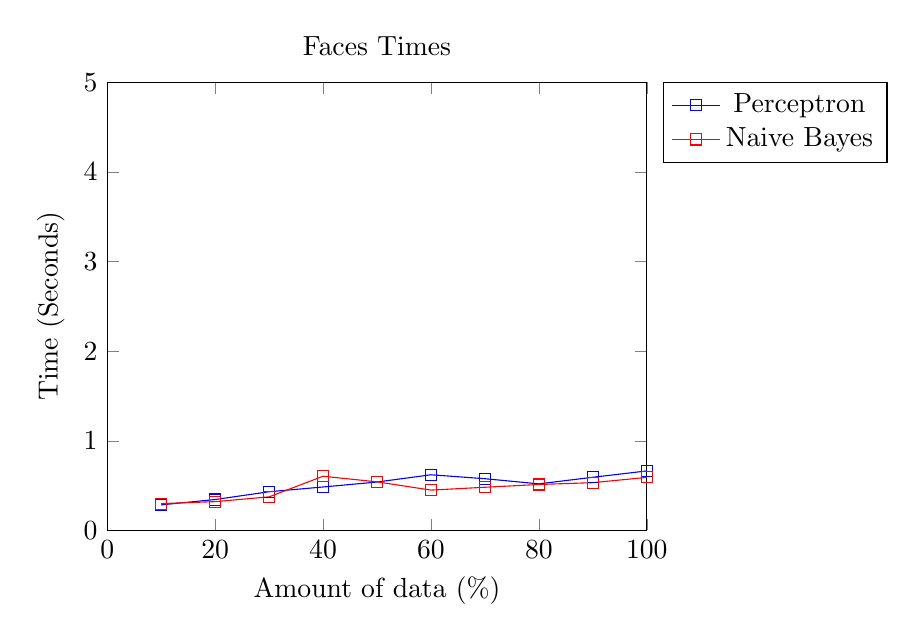
\begin{tikzpicture}
\begin{axis}[
  legend pos=outer north east,
  title={Faces Times}, 
  xlabel={Amount of data (\%)},
  ylabel={Time (Seconds)},
  xmin=0, xmax=100,
  ymin=0, ymax=5
  ]


  \addplot[
    color=blue,
    mark=square
  ]
  coordinates {
  (10,0.285628843307) (20,0.345379066467) (30,0.432191228867) (40,0.485308027267) (50,0.540548801422) (60,0.621487379074) (70,0.57750377655) (80,0.520122432709) (90,0.593709373474) (100,0.664348363876) 
  };
  \addplot[
    color=red,
    mark=square
  ]
  coordinates {
  (10,0.299941968918) (20,0.321775722504) (30,0.375074672699) (40,0.604894018173) (50,0.542614173889) (60,0.450457572937) (70,0.482290029526) (80,0.513176774979) (90,0.533605384827) (100,0.592084550858) 
  };
  \legend{Perceptron, Naive Bayes}

\end{axis}
\end{tikzpicture}

\subsubsection{Faces Std Dev}
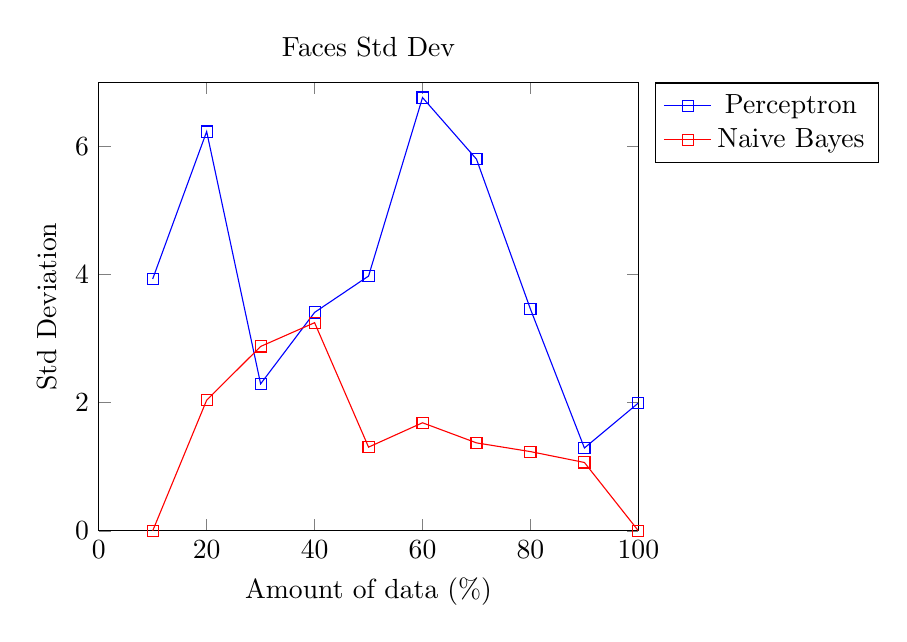
\begin{tikzpicture}
\begin{axis}[
  legend pos=outer north east,
  title={Faces Std Dev}, 
  xlabel={Amount of data (\%)},
  ylabel={Std Deviation},
  xmin=0, xmax=100,
  ymin=0, ymax=7
  ]

  \addplot[
    color=blue,
    mark=square
  ]
  coordinates {
  (10,3.932768321) (20,6.23395718803) (30,2.29395340454) (40,3.40978982735) (50,3.97771570405) (60,6.76461381012) (70,5.80268137253) (80,3.46153466287) (90,1.29271462864) (100,1.99555060628) 
  };
  \addplot[
    color=red,
    mark=square
  ]
  coordinates {
  (10,0.0) (20,2.03960780544) (30,2.87827108599) (40,3.24961536185) (50,1.30639452948) (60,1.68654808542) (70,1.37275068546) (80,1.23648246607) (90,1.06666666667) (100,0.0) 
  };
  \legend{Perceptron, Naive Bayes}

\end{axis}
\end{tikzpicture}
\section{Discussion and Conclusions}
One of the key differences that can be seen between these two algorithms is the rate of increase in the accuracy of the classifier as more training data is added. The naive bayes classifier benefited with more training data to a higher degree than the perceptron classifier. The perceptron classifier, as explained in section 3, started to plateau and sometimes even do worse as the training data was increased to above 40\% of the data available. \\ 
Another observation that can be seen is that the runtime is affected by the number of outputs that the classifier has to deal with. When classifying digits, the runtime for both classifiers was significantly higher, as there were 10 possible outputs, but was significantly faster when classifying faces, when there were only 2 possible outputs. On top of that, the classifiers had greater accuracy when there were less outputs. This is reasonable, since even if the classifier guessed the outputs at random, the probability of being correct increases as the number of choices decreases.\\ 
\end{document}
